\documentclass[a4paper,kulak]{kulakarticle}

\usepackage[utf8]{inputenc}
\usepackage[dutch]{babel}
\usepackage{pdfpages}
% style
\usepackage[left=2.5cm,top=2cm,right=2.5cm,bottom=2cm,a4paper]{geometry}
\usepackage{color}

% gantt
\usepackage{pgfgantt}
\usepackage{lscape}
\def\pgfcalendarweekdayletter#1{%
	\ifcase#1M\or T\or W\or T\or F\or S\or S\fi%
}


\definecolor{foobarblue}{RGB}{0,153,255}
\definecolor{foobaryellow}{RGB}{234,187,0}
\definecolor{grey}{RGB}{170,170,170}

\newganttchartelement{foobar}{
	foobar/.style={
		shape= rectangle,
		inner sep=0pt,
		draw=grey!70!blue,
		thick,
		fill=white,
		inner color=blue!10, outer color=blue!40, opacity=0.95
	},
	foobar incomplete/.style={
		/pgfgantt/foobar,
		draw=foobaryellow,
		bottom color=foobaryellow!50
	},
	foobar label font=\slshape,
	foobar left shift=0,%.1,
	foobar right shift=0%-.1
}


\date{\today}
\address{
	Bachelor in de fysica\\
	Bachelor in de informatica\\
	Bachelor in de wiskunde\\
	Ingenieurswetenschappen}
\title{BDA App}
\author{Marthe B\"{o}ting\\
	Robin Bruneel\\
	Toon Ingelaere}

\begin{document}
	\includepdf{voorblad}
	\newpage
	\maketitle
	\tableofcontents
	\newpage
	
	\section*{Inleiding}	
		Als gevolg van een bloedklonter in een hersenbloedvat ontstaat een ischemische beroerte. Deze klonter moet men zo snel mogelijk verwijderen dit kan met behulp van een geneesmiddel die de klonter oplost of door middel van mechanische verwijdering. Door deze mechanische verwijdering kan men de bloedklonter verder analyseren in het labo om een duidelijker beeld te krijgen.
		\newline
		Vandaag de dag verliest men zeer veel tijd aan het verwerken van de bloedklonters. Er is ons dan ook gevraagd om een app te ontwikkelen die de analyse van de foto’s volledig automatisch kan uitvoeren.
		\newline
		In dit verslag gaan we eerst in op wat de klant specifiek van ons verwacht en aan welke specificaties ons ontwerp moet voldoen. Hierna gaan we ons design bespreken en toelichten. Verder bespreken we ook onze voorlopige resultaten. Ten slotte wordt er nog een blik geworpen naar de vakken uit eerste 3 semesters die ons hierbij geholpen hebben.
	
	\section{Klantenvereisten}
		De klant verwacht een gebruiksvriendelijke app waarbij hij een foto kan ingeven en dat deze automatisch bewerkt wordt. De foto moet  worden bijgesneden en de achtergrond moet verwijderd worden. Daarnaast is het de bedoeling om de bloedklonter te analyseren met andere woorden het berekenen van het percentage van een eiwit. Dit gebeurt door een hoeveelheid kleur te quantificeren in de bloedklonter. 
	
	\section{Ontwerpspecificatie}
		De klant wil een app die elke foto kan bijwerken en ook een percentage van de eiwitten weergeven. Er zijn geen verdere voorwaarden verbonden aan de grootte van de foto. Een absolute voorwaarde om de foto bij te snijden is dat de bloedklonter er volledig opstaat. Desondanks mag de rand niet te groot zijn omdat dit anders te veel geheugen in beslag neemt. De achtergrond moet volledig wit gemaakt worden zodat er geen fouten worden gemaakt bij het berekenen van een hoeveelheid kleur. De app moet voor iedereen bruikbaar zijn. Daarnaast moeten de verschillende foto's over de verschillende fasen getoond worden.
		
	\section{Onze oplossing}

		\subsection{Achtergrondverwijdering}
			Het eerste deel van ons project is de achtergrond van de bloedklonters te verwijderen. Op de afbeeldingen is er heel wat vuiligheid te vinden. Een voorbeeld hiervan zijn luchtbellen of kleine bloedklonters zoals men ziet op de volgende figuur \ref{figuur achtergrondverwijdering}. Hieronder zullen we verschillende operaties beschrijven om de grootste klonters te lokaliseren en alles dat geen klonter is te verwijderen. Dit leidt tot een ruisvrije afbeelding.

		\begin{figure}[H]
		\centering
		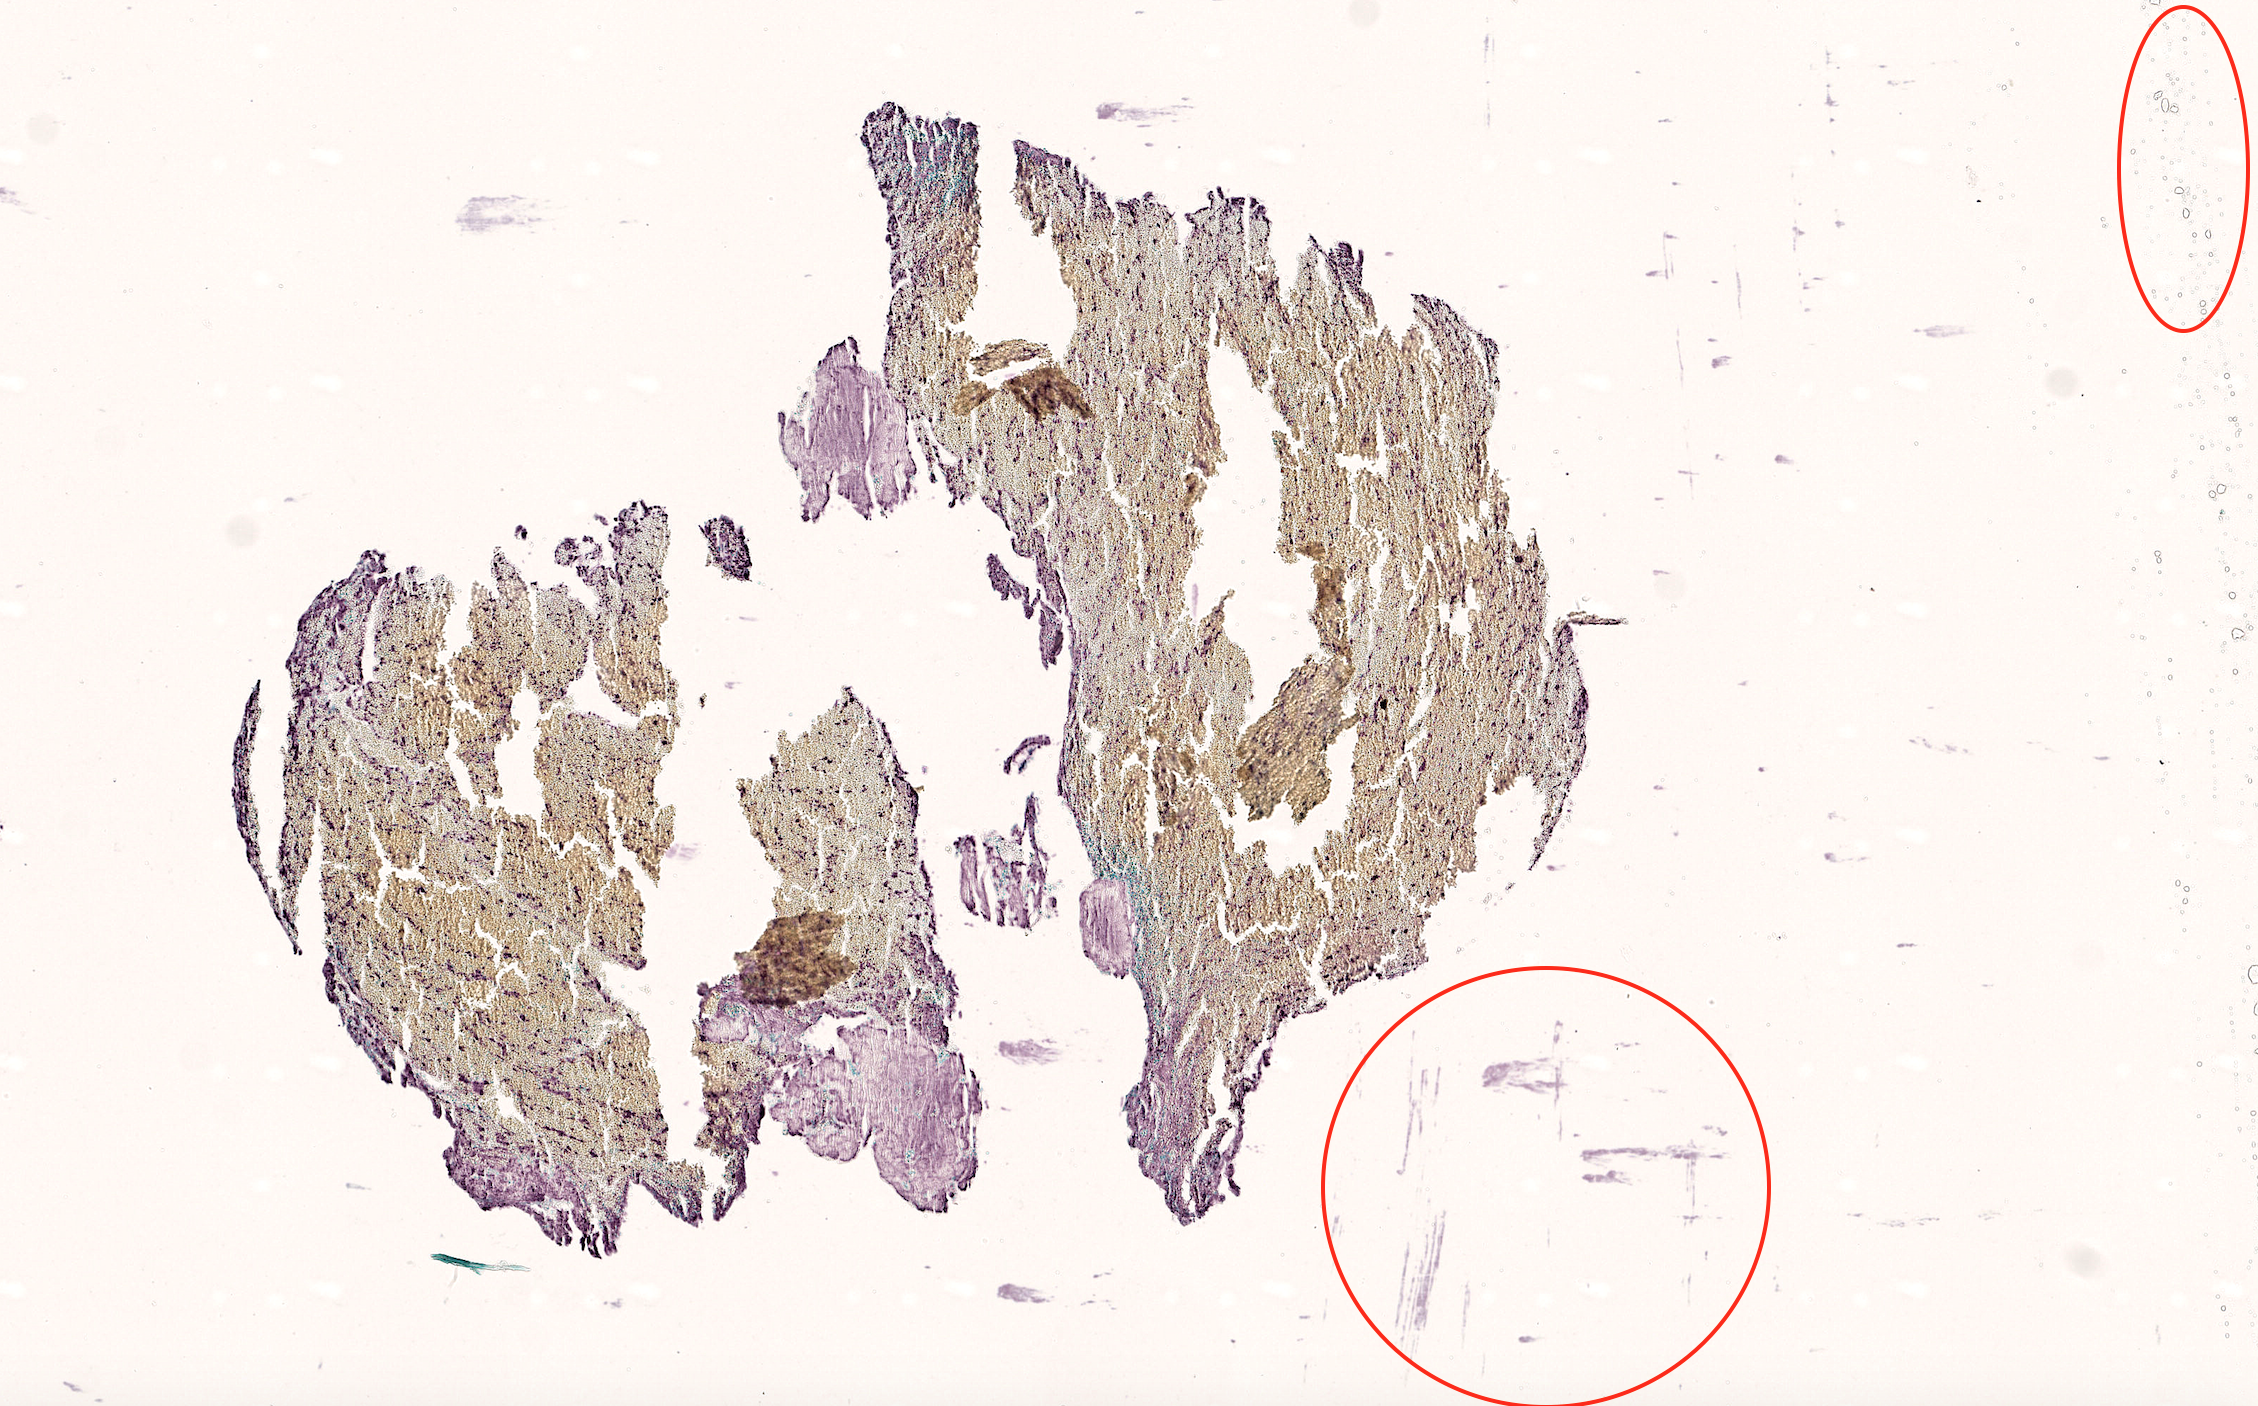
\includegraphics[width = \textwidth]{Ruis_afbeelding.png}
	
		\caption{In de rechterbovencirkel zien we luchtbellen en in de onderste cirkel zien we een verkleuring die geen deel uitmaakt van een bloedklonter.}
		\label{figuur achtergrondverwijdering}
		\end{figure}

	\subsubsection{Bepalen van de beste treshold}
		Wanneer we de grijswaarden van de afbeelding berekenen, zien we een duidelijk verschil tussen de achtergrond (eerder wit) en de bloedklonter (eerder grijs) zoals we zien op figuur \ref{figuur beste_treshold}. Wanneer we een histogram van deze grijswaarden opstellen, vinden we ook dat er een lokaal minimum is tussen het grijs en het wit. Dit zien we duidelijk op het histogram \ref{figuur graf1}. Wanneer we dit minimum berekenen vinden we de theoretisch optimale treshold, de waarde om een bloedklonterpixel van een achtergrondpixel te onderscheiden. Wanneer we die treshold toepassen en een binaire representatie zoals figuur \ref{figuur foto_bin} vormen, zien we duidelijk dat dit een goede treshold is.

	\begin{figure}[H]
	\centering
	\subfloat[]{{\includegraphics[height=8cm]{origineel_vb}}}
	\subfloat[]{{\includegraphics[height=8cm]{grijswaarden_vb}}}
	
	\caption{Illustratie van de originele foto (a) en deze omgezet in grijswaarden (b)}
	\label{figuur beste_treshold}
	\end{figure}

	\begin{figure}[H]
	\centering
	\includegraphics[width=0.85\textwidth]{GetBestTreshold_vb_aangeduid.png}
	
	\caption{Histogram van het aantal pixels gegroepeerd per grijswaarde. We zien duidelijk een lokaal minimum rond de waarde 230. Opmerking: we maken hier gebruik van een logaritmische y-as.}
	\label{figuur graf1}
	\end{figure}

	\begin{figure}[H]
	\centering
	\includegraphics[width=0.7\textwidth]{grijswaarden_bin_vb}
	\caption{Op deze binaire representatie zijn de bloedklonters duidelijk te zien}
	\label{figuur foto_bin}
	\end{figure}

	\subsubsection{Lokaliseren van de bloedklonters}
		Eenmaal deze binaire representatie gevonden is, lokaliseren we de grootste klonters om het ruis te verwijderen. Hiervoor zullen we eerst alle holtes in de klonters opvullen door alle ingesloten pixels\footnote{Een ingesloten pixel is een zwarte pixel die onmogelijk de achtergrond van de afbeelding kunnen bereiken zonder over witte pixels te gaan} wit te maken. Het resultaat is te zien in figuur \ref{figuur lok_bloed}. De klonters zijn nu nog veel duidelijker zichtbaar, waardoor we kunnen overgaan naar de effectieve ruisfilter.

	\begin{figure}[H]
	\centering
	\includegraphics[width = 0.7\textwidth]{grijswaarden_bin_gevuld_vb}
	\caption{Alle gaatjes zijn nu opgevuld, waardoor we de grootte van de bloedklonters kunnen berekenen}
	\label{figuur lok_bloed}
	\end{figure}

	\subsubsection{Ruisfilter}
		Voor de ruisfilter verwijderen we elke groep witte pixels met een omvang kleiner dan een constante waarde. Indien dit zo is, worden de witte pixels door zwarte vervangen. Dit simpel algoritme verwijdert alle ruis zoals te zien is in figuur \ref{figuur ruisfilter}. Deze zogenaamde 'mask' kunnen we toepassen op de originele afbeelding om officieel het ruis te verwijderen.

	\begin{figure}[H]
	\centering
	\subfloat[]{{\includegraphics[width=8cm]{ruisvrij_vb}}}
	\subfloat[]{{\includegraphics[width=8cm]{ruisvrij_kleur_vb}}}
	
	\caption{Alle ruis is verwijderd, dit is een foto waarmee we kunnen werken}
	\label{figuur ruisfilter}
	\end{figure}

	\subsection{Lokalisatie van de indicator}
		Het tweede deel van ons project is de indicators lokaliseren. We hebben de opdracht gekregen twee soorten te kunnen onderscheiden. Een voorbeeld van deze twee is op de volgende figuren \ref{figuur indicators} te zien. Omdat het kleurverschil tussen indicator en achtergrond niet altijd even groot is, vormen we het oorspronkelijke \textit{RGB} kleurmodel \footnote{Het RGB kleurmodel is een voorstelling waarbij ieder kleur voorgesteld wordt door een waarde van de drie basiskleuren(rood, groen en blauw)} om naar het zogenaamde \textit{HSV} kleurmodel. Dit model is een alternatieve voorstelling waarbij men alle kleuren op een cirkel voorstelt, de hoek die dit kleur maakt, noemt men de \textit{Hue}. Naast deze waarde heeft \textit{HSV} nog twee andere parameters namelijk \textit{Saturation} en \textit{Value}. \textit{Saturation} kan simpel beschouwd worden als een aanduiding van de hoeveelheid witte kleur en \textit{Value} een aanduiding van de zwarte kleur. Een grafisch overzicht is te zien op figuur \ref{figuur hsv_schema}.\\
		Het voordeel van deze transformatie is dat het heel wat eenvoudiger is om een onderscheid tussen dichtbijgelegen kleuren te vinden. Een andere mogelijke transformatie is die naar het \textit{Lab} kleurmodel die gelijkaardige eigenschappen heeft en desnoods ook gebruikt kan worden. Eenmaal we een duidelijk onderscheid tussen de indicator en de achtergrond maken, kunnen we eenvoudig het percentage indicator berekenen door het aantal bloedklonter- en indicatorpixels op te tellen. Ons stappenplan wordt in volgende hoofdstukken besproken en wordt toegepast op de afbeelding uit figuur \ref{figuur indicators} (a).
	
	\begin{figure}[H]
	\centering
	\subfloat[]{{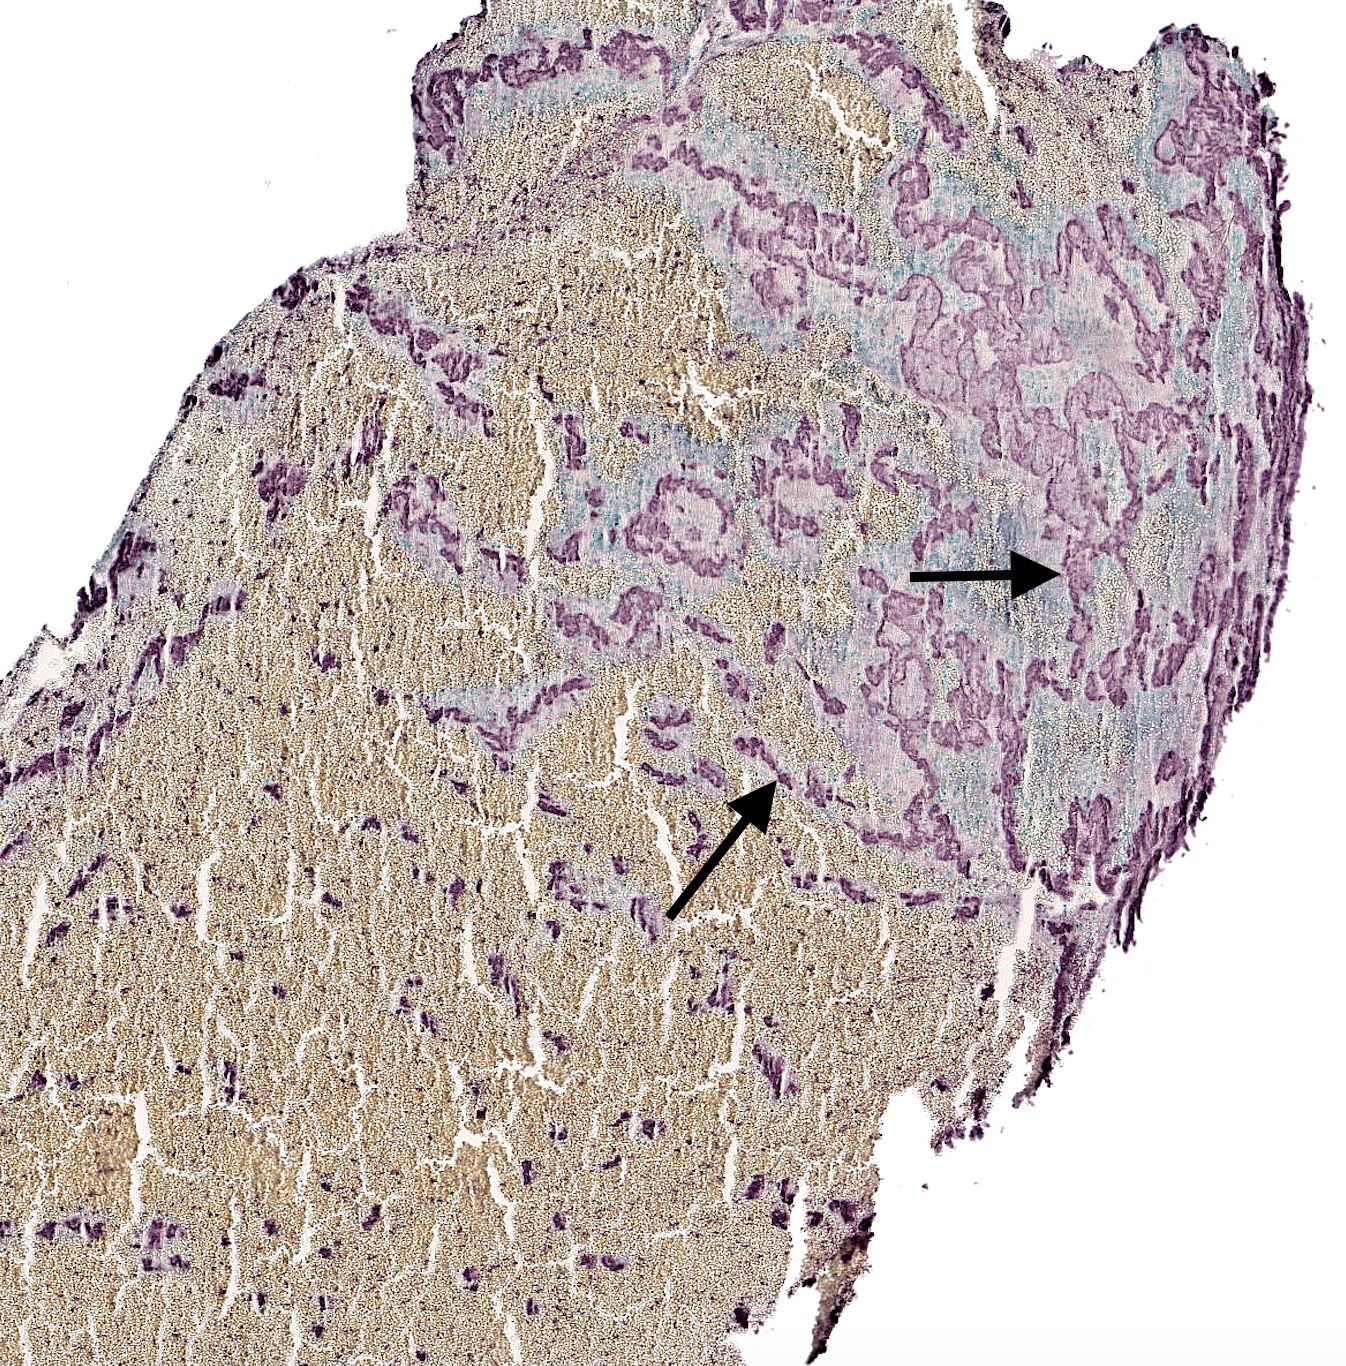
\includegraphics[width=7.5cm]{Indicator_vb1}}}
	\qquad
	\subfloat[]{{\includegraphics[width=7.5cm]{Indicator_vb2}}}
	
	\caption{Illustratie van de twee soorten indicator (respectievelijk paars en donkerroze) die gedetecteerd moeten worden. We zien duidelijk dat het detecteren op afbeelding (a) eenvoudiger zal zijn dan op afbeelding (b)}
	\label{figuur indicators}
	\end{figure}

	\begin{figure}[H]
	\centering
	\includegraphics[width=0.7\textwidth]{HSV_vb.png}
	
	\caption{Grafische voorstelling van het HSV (Hue, Saturation, Value) kleurmodel}
	\label{figuur hsv_schema}
	\end{figure}

	\subsubsection{het HSV kleurmodel}
		Zoals reeds vermeld, beginnen we met een transformatie naar het \textit{HSV} kleurmodel. Bijgevolg kunnen we de twee voorstellingen vergelijken. We hebben het model telkens ontbonden in de drie kleurwaarden, waarbij zwart de laagste waarde voor dat kleur is en wit de hoogste. De resultaten zijn te zien in de figuren \ref{figuur RGB} en \ref{figuur HSV}. Het verschil tussen de twee kleurmodellen is duidelijk te zien, afbeelding (a) en (b) uit figuur \ref{figuur HSV} lijken namelijk iets agressiever een onderscheid tussen de kleuren te maken.

	\begin{figure}[H]
	\centering
	\subfloat[]{{\includegraphics[width=4.5cm]{RGB_r}}}
	\qquad
	\subfloat[]{{\includegraphics[width=4.5cm]{RGB_g}}}
	\qquad
	\subfloat[]{{\includegraphics[width=4.5cm]{RGB_b}}}
	\caption{Illustratie van respectievelijk de rode, groene en blauwe kleurwaarden (RGB). Hierbij komt wit overeen met de maximumwaarde en zwart met de minimumwaarde van die kleur.}
	\label{figuur RGB}
	\end{figure}

	\begin{figure}[H]
	\centering
	\subfloat[]{{\includegraphics[width=4.5cm]{HSV_h}}}
	\qquad
	\subfloat[]{{\includegraphics[width=4.5cm]{HSV_s}}}
	\qquad
	\subfloat[]{{\includegraphics[width=4.5cm]{HSV_v}}}
	
	\caption{Illustratie van respectievelijk de hue, saturation en value kleurwaarden (HSV). Hierbij komt wit overeen met de maximumwaarde en zwart met de minimumwaarde van die kleurwaarde.}
	\label{figuur HSV}
	\end{figure}

	\subsubsection{Een algemene treshold}
		De volgende stap is nu een filter bepalen voor alle indicatorpixels. Het probleem is echter dat een goede filter voor de ene foto niet altijd een goede filter voor de andere foto is. Daarom hebben we voor iedere foto manueel een 'treshold' bepaald en deze achteraf met elkaar vergeleken. Het resultaat is een vrij algemene treshold die alle indicatorpixels met zekerheid aanduidt. Af en toe worden jammer genoeg verkeerde pixels aangeduid. Het aantal is weliswaar niet zo groot, maar zullen we trachten te omzeilen in het volgende hoofdstuk. Een voorbeeld van deze algemene treshold is te zien op de volgende figuur \ref{figuur alg_tresh}

	\begin{figure}[H]
	\centering
	\includegraphics[width = 0.7\textwidth]{algemene_treshold}
	
	\caption{We hebben alle indicatoren met een blauwachtige kleur aangeduid. De algemene treshold selecteert alle indicatorpixels, maar jammer genoeg ook enkele verkeerde (voornamelijk rechtsonder).}
	\label{figuur alg_tresh}
	\end{figure}

	\subsubsection{Optimalisatie van de treshold}
		In dit hoofdstuk willen we het aantal verkeerde pixels verminderen zonder de juiste te beïnvloeden. We hebben echter al een vrij goede treshold waardoor we een statistische analyse van wat onder deze mask ligt, kunnen uitvoeren. We stellen hiervoor een frequentiediagram van de \textit{HSV} kleurwaarden onder de mask op. Het levert ons namelijk een interessant resultaat dat te zien is in figuur  \ref{figuur HSVHIST}. We zien namelijk duidelijke verschillen in de frequenties van de kleurwaarden. \\
		Het idee is om nu de verkeerde pixels via deze diagrammen eruit te filteren. Indien we veronderstellen dat de frequenties van deze specifieke pixels laag zijn en dat de verkeerde pixels in kleur verschillen met de indicatorpixels. Dan kunnen we in principe alle pixels met een frequentie onder een bepaalde grenswaarde schrappen. Een betere benadering is misschien om het punt te vinden, waar de frequentie van de pixels enorm begint toe te nemen of we met andere woorden grote 'indicatoraders' aan het verwijderen zijn. Dit punt kan theoretisch benaderd worden als het maximum van de tweede afgeleide naar de kleurwaarde. Jammer genoeg hebben we de tijd nog niet gehad om dit idee te testen. \\
		Een mogelijk extra stap is om de indicatorpixels morfologisch te sluiten met een algoritme dat reeds in MATLAB verwerkt is. Indien we met onze filtering enkele holtes maken, kunnen deze dan zonder problemen worden opgevuld. Ter illustratie geven we het standaardvoorbeeld van MATLAB in figuur \ref{figuur morf} weer.


	\begin{figure}[H]
	\centering
	\subfloat[]{{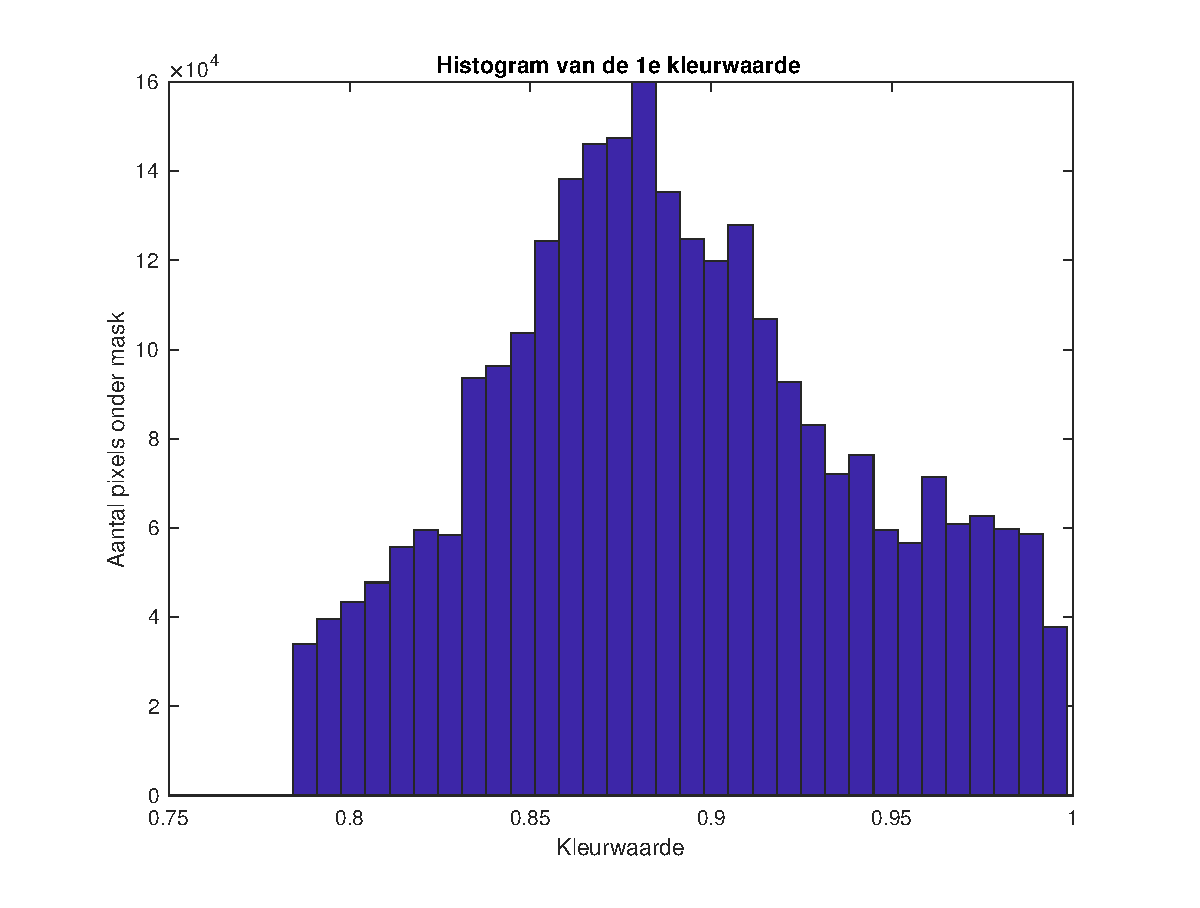
\includegraphics[width=4.5cm]{hsvhist_h}}}
	\qquad
	\subfloat[]{{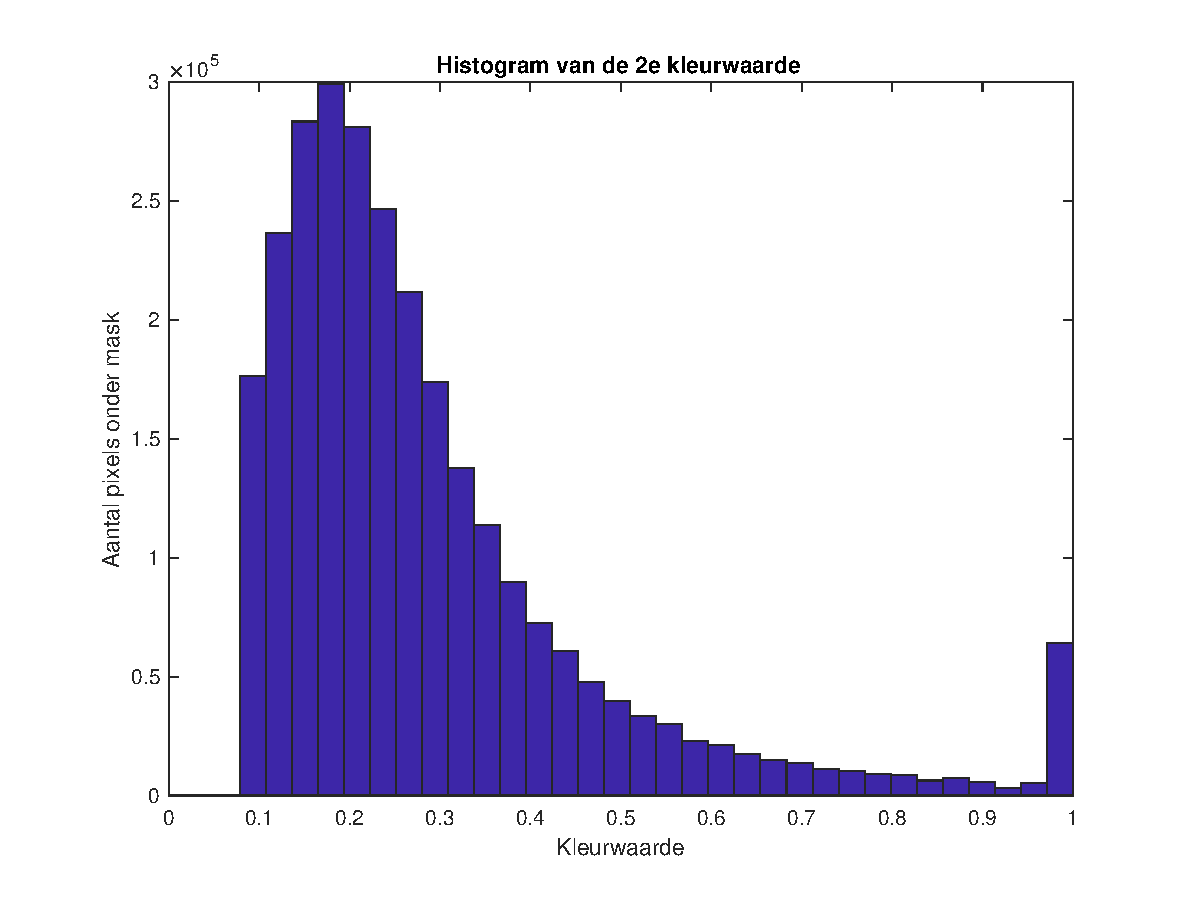
\includegraphics[width=4.5cm]{hsvhist_s}}}
	\qquad
	\subfloat[]{{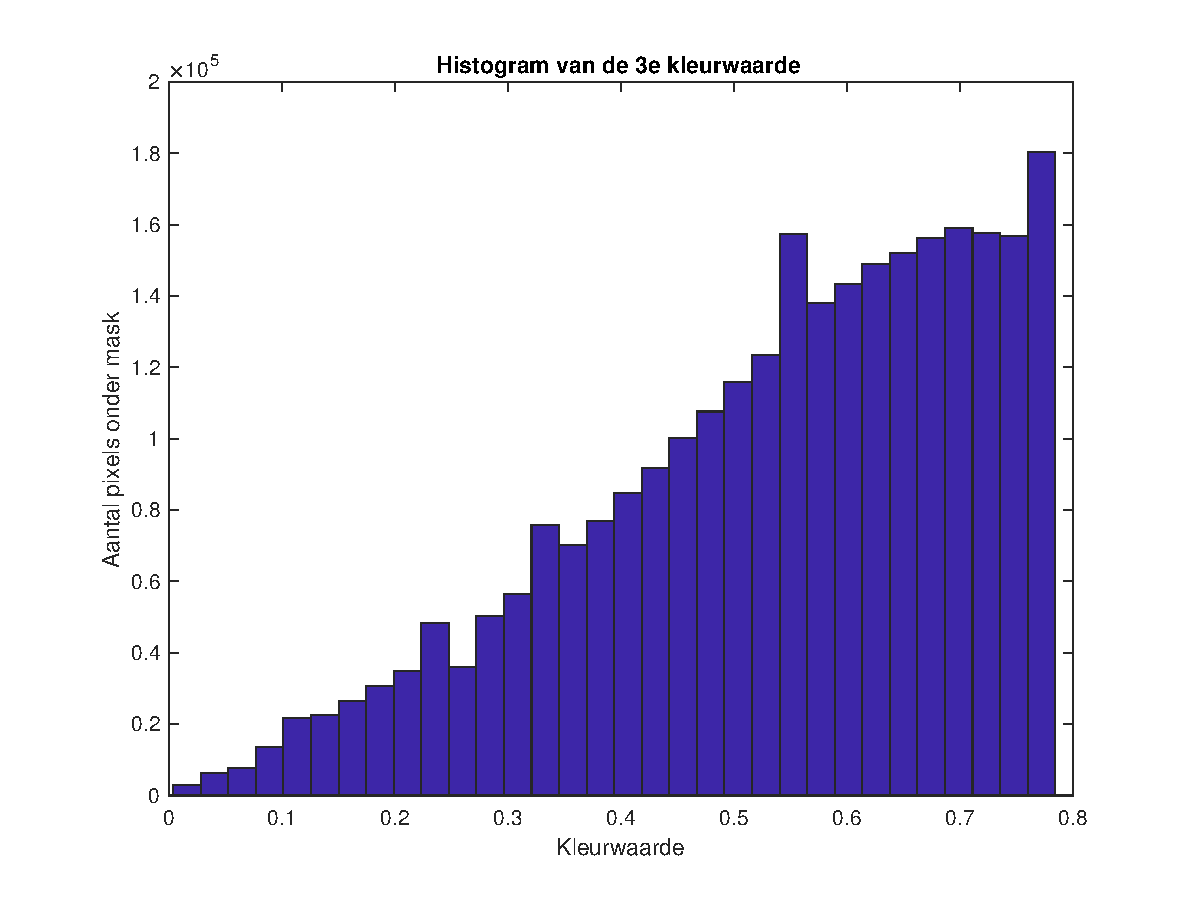
\includegraphics[width=4.5cm]{hsvhist_v}}}
	
	\caption{Histogrammen van de HSV kleurwaarden. We zien duidelijk het verschil in frequenties}
	\label{figuur HSVHIST}
	\end{figure}

	\begin{figure}[H]
	\centering
	\subfloat[]{{\includegraphics[width=7.5cm]{morf_open}}}
	\qquad
	\subfloat[]{{\includegraphics[width=7.5cm]{morf_gesloten}}}
	
	\caption{Illustratie waarbij de witte cirkels uit afbeelding (a) morfologisch gesloten worden in afbeelding (b)}
	\label{figuur morf}
	\end{figure}

	\subsection{De gebruiksvriendelijke applicatie}
		Momenteel zijn dit nog afzonderlijke programma's waarbij we steeds zelf de te aan te passen foto erin inzetten. Naar de klant toe is dit geen manier van werken en wordt dit in een app samengebracht. De klant zal dan zelf kunnen ingeven welke foto hij wil laten verwerken. Eénmaal de foto gekozen is , zal in de eerste fase de achtergrond van de foto wit worden gemaakt en zal de foto afgesneden worden zodanig dat enkel de bloedklonter zichtbaar is. Als dit gebeurd is , zal er al een eerste resultaat getoond worden. Hierdoor heeft de klant een beeld waarop de verdere analyse zal gebeuren en kan die eventueel ingrijpen bij fouten. Vervolgens zal de kleurenanalyse gebeuren. Ook hiervoor zal de foto getoond worden waarop de klant kan zien welke delen de indicator bevatten en zal het percentage gegeven worden. De basis van de app hebben we al zoals te zien is in  figuur \ref{fig: app}
	
		\begin{figure}[H]
		\centering
		\includegraphics[width=170mm]{app.jpg}
		\caption{Voorstelling van de app}
		\label{fig: app}
		\end{figure}
	
		
	

	\section{Voorlopige resultaten}		
		Op dit moment kunnen we al effectief de foto gebruiksklaar maken voor de analyse ervan. Dit houdt in dat we alle pixels die niet tot de bloedklonter behoren wit kunnen maken en de afbeelding zodanig kunnen bijsnijden dat er geen overbodig geheugen ingenomen wordt door de afbeelding. In Figuur \ref{fig: voorna} wordt dit geïllustreerd.\\
	
		\begin{figure}[H]
		\centering
		\subfloat[Afbeelding van bloedklonter voor die bewerkt wordt]{{\includegraphics[width=4.5cm]{BloedklonterVoor.jpg}}}
		\qquad
		\subfloat[Bijgesneden afbeelding van de Bloedklonter met witte achtergrond ]{{\includegraphics[width=4.5cm]{BloedklonterNa.jpg}}}
		
		\caption{Illustratie van hoe we de afbeelding gebruiksklaar maken voor de analyse ervan}
		\label{fig: voorna}
		\end{figure}
		
		
		Momenteel zijn we bezig met de implementatie van de kleurendetectie. We hebben hier al veel vooruitgang geboekt, maar de hij staat nog niet volledig op punt. Ook hebben we al even geëxperimenteerd met de app designer van Matlab. Hier willen we namelijk onze gebruiksvriendelijke applicatie in maken.
		Op basis van wat we nu al bereikt hebben, denken we dat dit project een succes kan worden en dat men het effectief zal kunnen gebruiken in het onderzoek naar de samenstelling van bloedklonters.
	
	\section{Verantwoordelijkheden en taakverdeling}		
		In onze groep hebben we ervoor gekozen om Robin aan te stellen als projectleider. Hij verdeelt elke week de taken en heeft het laatste woord bij discussies. 
		Voor de verslagen en de eindpresentatie is Marthe verantwoordelijk. Zij is de eindredactrice van alle verslagen. We schrijven de verslagen uiteraard samen, maar het is haar taak ervoor te zorgen dat deze volledig en gestructureerd zijn en dat ze voor de deadline ingediend worden.\\
		Voor de implementatie van de code zijn we elk verantwoordelijk voor ons eigen deel. Zo wordt het verwijderen van de ruis en het bijsnijden van de afbeelding door Toon geleid, de kleurdetectie door Robin en de implementatie van de app door Marthe.
		
	\section{Integratie met vakken uit eerste 3 semsters}
		Om dit probleem op te lossen hebben we gebruik gemaakt van matlab. Het is dan ook een meerwaarde dat we in het eerste semester 'beginselen van programmeren' gehad hebben waardoor we sneller vertrouwd geraken met deze programmeertaal. Daarnaast leren we in 'nummerieke wiskunde' ook werken met matlab. Statistische analyse gebruiken we voor het analyseren van de verschillende kleuren.
	
	\section{Besluit}	
		Momenteel kunnen we besluiten dat we goed aan het vorderen zijn. Zoals eerder vermeld kunnen we de foto automatisch bijsnijden en de achtergrond ruisvrij maken. Onze focus ligt nu voornamelijk bij de implementatie van de kleurendetectie. Eénmaal deze ook op punt staat kunnen we beide programma's in de app steken en deze optimaliseren met de nadruk op gebruiksvriendelijkheid naar de klant toe. Verder houden we de klant op de hoogte over onze vooruitgang via onder andere dit verslag. 

	\newpage		
	
	

		\begin{landscape}
			\flushleft
			\begin{ganttchart}[hgrid, vgrid, x unit=5mm,y unit title=1cm,
				y unit chart=1cm, time slot format=isodate]{2018-09-24}{2018-11-04}
				\gantttitlecalendar{week,month=shortname,day,weekday=letter} \\	
			
				\ganttfoobar{1}{2018-10-04}{2018-10-18}\\
				\ganttfoobar{2}{2018-10-11}{2018-11-01}\\
				\ganttfoobar{3}{2018-10-18}{2018-11-04}\\
				\ganttgroup{}{2018-10-18}{2018-11-01}
				\ganttmilestone{T.T. verslag}{2018-11-02}\\
			
			
			\end{ganttchart}
		
			\begin{ganttchart}[hgrid, vgrid, x unit=5mm,y unit title=1cm,
				y unit chart=1cm, time slot format=isodate]{2018-11-05}{2018-12-23}
				\gantttitlecalendar{week,month=shortname,day,weekday=letter} \\
			
				\ganttfoobar{3}{2018-11-05}{2018-11-15}\\
				\ganttfoobar{4}{2018-11-08}{2018-12-06}\\
				\ganttgroup{}{2018-11-29}{2018-12-17}
				\ganttmilestone{Eindverslag}{2018-12-18}\\
				\ganttmilestone{Eindpres.}{2018-12-20}\\			
			
			\end{ganttchart}
		\end{landscape}
	
		\begin{table}
			\centering
			\begin{tabular}{c|l}
				\textbf{Taaknummer} & \textbf{Taakomschrijving}\\
				\hline
				\textbf{1} & Achtergrond verwijderen en afbeelding bijsnijden\\
				\textbf{2} & Kleuren detecteren en kwantificeren\\
				\textbf{3} & Ontwerpen van een gebruikersvriendelijke app\\
				\textbf{4} & Optimalisatie van het algoritme\\
			\end{tabular}
			\caption{Omschrijvingen van de taken in de gantt-chart}
			\label{ganttcharttabel}
		\end{table}

\end{document}
